\documentclass[12pt,a4paper]{scrartcl}

\usepackage{hyperref}
\usepackage{url}
\usepackage{graphicx}
\usepackage{xcolor}
\usepackage{textcomp}
\usepackage{subfig}

\newcommand{\obtain}[0]{\textcolor{orange}{\textbf{obtain}}}
\newcommand{\avail}[0]{\textcolor{green}{\textbf{available}}}
\newcommand{\build}[0]{\textcolor{red}{\textbf{build}}}
\newcommand{\code}[0]{\textcolor{blue}{\textbf{code}}}
\newcommand{\hack}[0]{Hack`a'thing}
\newcommand{\gasometer}[0]{\texttt{Gas`o'meter}}
\newcommand{\ph}[0]{h{\small$^{-1}$}}
\newcommand{\ox}[0]{O$_2$}
\newcommand{\cox}[0]{CO$_2$}

\parskip 0.3 cm
\parindent 0 cm

\title{1$^{st}$ QTB PBR \hack{}}
\subtitle{Soldering for and by beginners.}
\date{March 2--4, 2016}

\begin{document}
\maketitle
%\scriptsize
\tableofcontents
%\normalsize
\newpage

\section{PBR \hack{} Projects}
\label{proj}

\begin{figure}[ht]
  \begin{minipage}{.49\textwidth}
    \subfloat[Dougie's Reactor]{
      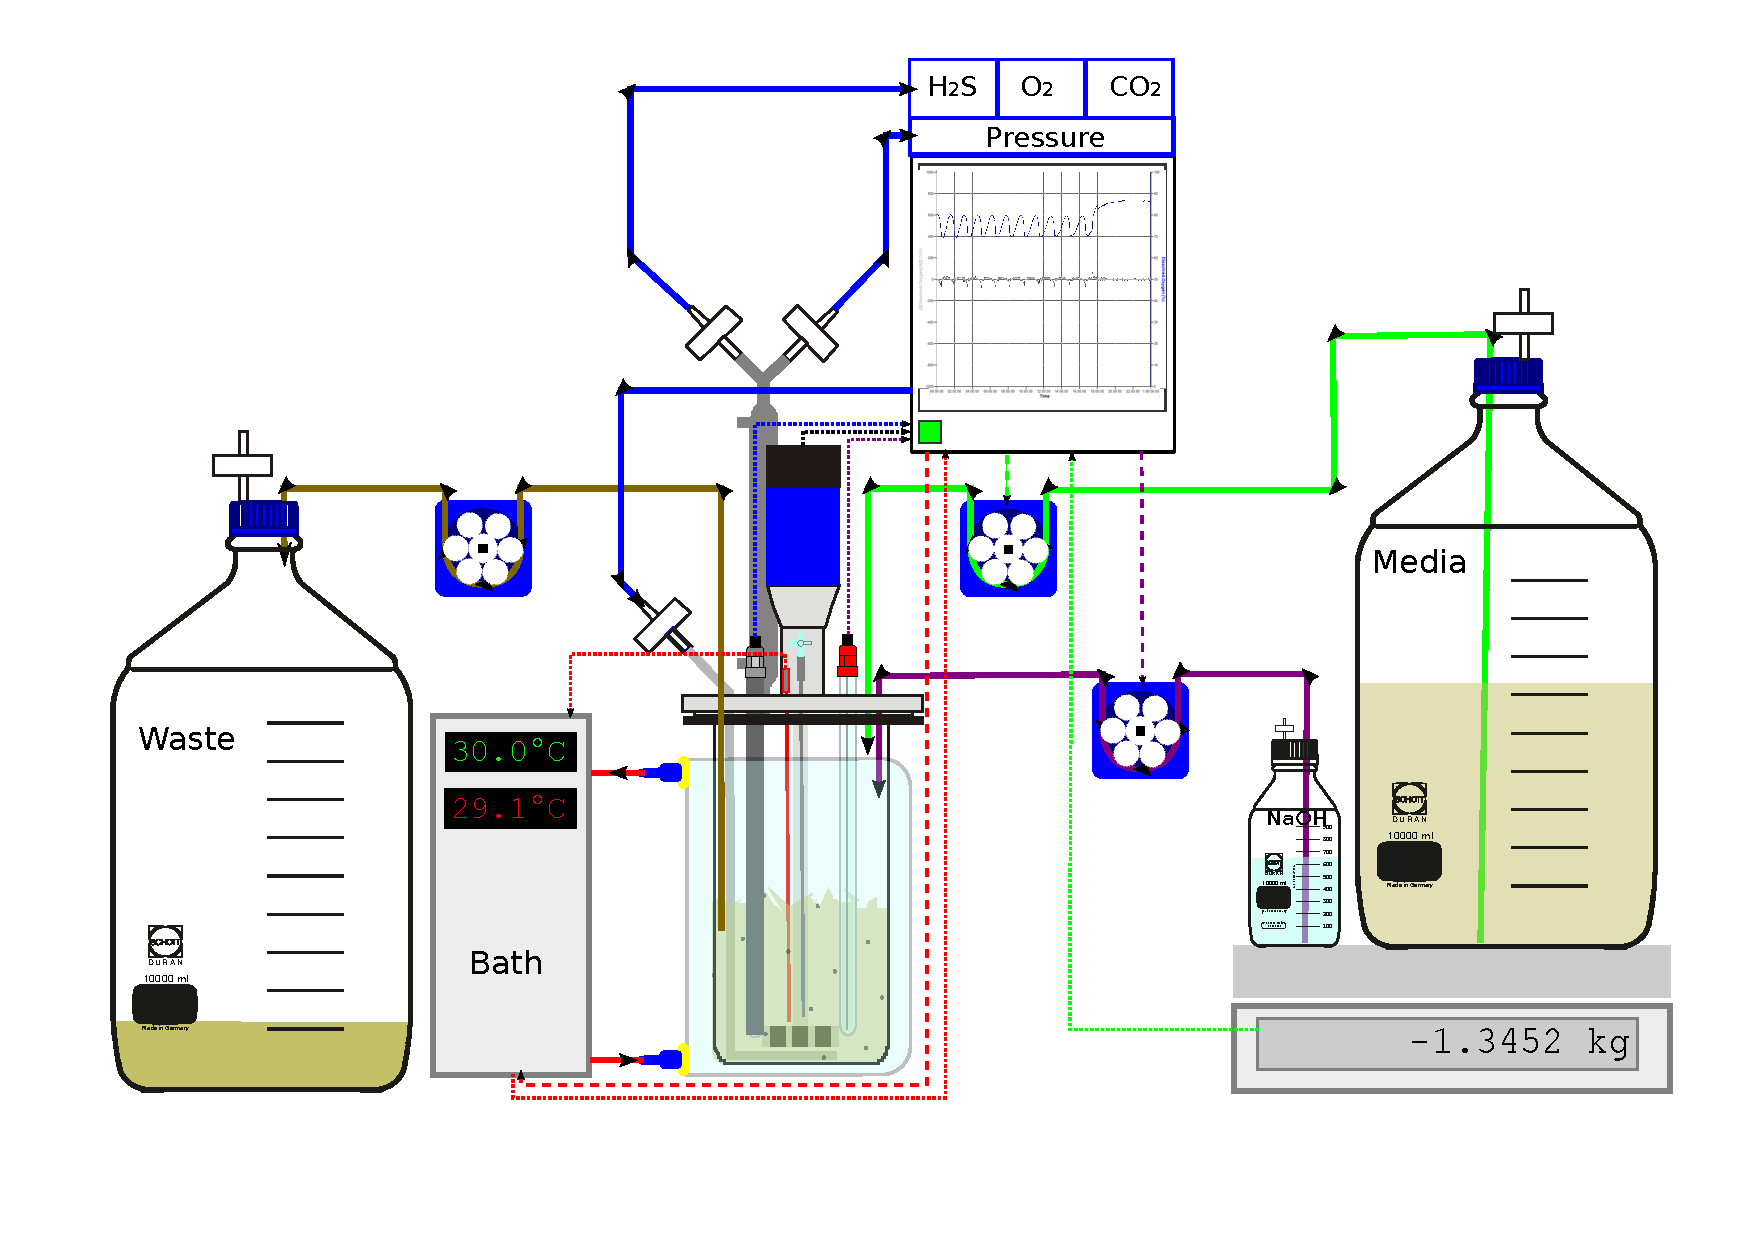
\includegraphics[width=\textwidth]{figures/fermentor_detailed.pdf}\\ 
    }
  \end{minipage}
  \begin{minipage}{.49\textwidth}
    \centering Monod: $\mu = \mu_{max} \frac{S}{S+K_S}$\\
    \subfloat[Snoep \textit{et al.} 2009]{
      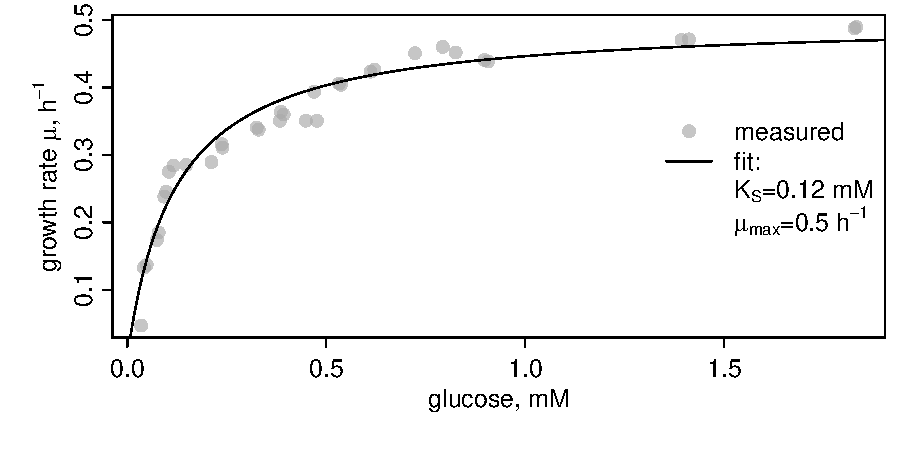
\includegraphics[width=\textwidth]{figures/snoep09_fig2.pdf}
    }
  \end{minipage}
\caption[]{Bioreactors}
\end{figure}



\newpage
\subsection{Gas Flux: \gasometer{}}
\label{gas}
\paragraph{Project:} 
Extend existing setup, co2meter's
\href{http://www.co2meter.com/collections/co2-sensors/oxygen-sensors}{\ox{}}
and
\href{http://www.co2meter.com/collections/co2-sensors/products/cozir-5-100-co2-sensor}{\cox{}}
sensors with Sainsmart's
\href{http://www.sainsmart.com/featured-products/sainsmart-mega2560-board-3-5-tft-lcd-module-display-shield-kit-for-atmel-atmega-avr-16au-atmega8u2.html}{Arduino
  Mega+Touch screen}

\begin{enumerate}
\item \code{} sensor calibration routines via touch-screen (use PSI
  gas mixing system)
\item \build{} water trap, tubing path from reactor, and casing for
  sensors and Arduino; \build{} improved gassing system (glas
  blowers!) to allow lower flow
\item \build{} \& \code{} interface to \href{http://www.aalborg.com/index.php/main_page/product_overview/id_product_overview/63}{Aalborg XFM digital mass flow
  meter}: connect the Aalborg's RS 485 interface to Arduino hardware
  serial Tx3/Rx3, and Ground
\item \build{} \& \code{} valve control to measure several reactors;
  connect via Arduino software serial connections; perhaps attach to
  PSI Multicultivator
\end{enumerate}

\paragraph{Ressources:}
\begin{itemize}
\item Sensor manuals in \texttt{manuals/offgas/} at
  \url{https://git.hhu.de/machne/PSIControl}:
  \texttt{Manual-CM-0201-UV-Flux-Oxygen.pdf},
  \texttt{Manual-GSS-Sensors.pdf}, and\\
  \texttt{A\_XFM\_Manual\_TD0701M[...].pdf}
\item Code in  \texttt{offgas/arduino/} at
  \url{https://git.hhu.de/machne/PSIControl} 
\end{itemize}

\paragraph{Materials:}

\begin{itemize}
\item Existing setup: \avail{}
\item Aalborg XFM, with RS 485 interface: \avail{}
\item Valve system for gas tubing, controllable \textit{via} serial
  interface: \obtain{}
\end{itemize}

\newpage
\subsection{Light Flux: Spectrometer} 
\label{spec}
\paragraph{Project:} 
Simple spectrometric measuring tool based on
\href{http://www.avantes.com/products/spectrometers/compactline/item/723-avaspec-mini}{AvaSpec-Mini2048l-V25}

\begin{enumerate}
\item Basic: Connect to Rasperry Pi, using drivers provides by
  Avantes; \code{} simple interface with display and/or recording
  functions
\item Advanced: use LED for absorbance, reflectance, or fluorescence
  measurements; \build{} light paths and perhaps a reactor probe for
  online recording
\end{enumerate}

\paragraph{Ressources:}
\begin{itemize}
\item
  \href{http://www.avantes.com/images/productsheets/AvaSpec_Mini5.pdf}{AvaSpec-Mini
    data sheet} in \texttt{manuals/spectrometer/} at
  \url{https://git.hhu.de/machne/PSIControl}
\end{itemize}

\paragraph{Materials:}
\begin{itemize}
\item AvaSpec-Mini2048l-V25, Minispectrometer: \avail{}\\ Mini
  spectrometer, 2048 Large pixels, grating-MN0600-0.50 (350-885nm),
  OSC, 25\textmu{}m slit, USB2 interface, AvaSoft-Basic
\item Fiber optic cables, VIS/NIR: 1 m, 200 \textmu{}m VIS/NIR and 1m,
  600 \textmu{}m: \avail{}\\
  SMA terminations, metal protection sleeves
\item Raspberry Pi Version 1: \obtain{}
\item LED system: use PSI LEDs or \obtain{}
\item Reactor probe: \build{} together with fine mechanics or glas
  blowers
\end{itemize}

\begin{figure}[ht]
  \begin{minipage}{.49\textwidth}
    \subfloat[AvaSpec-Mini 2048]{
      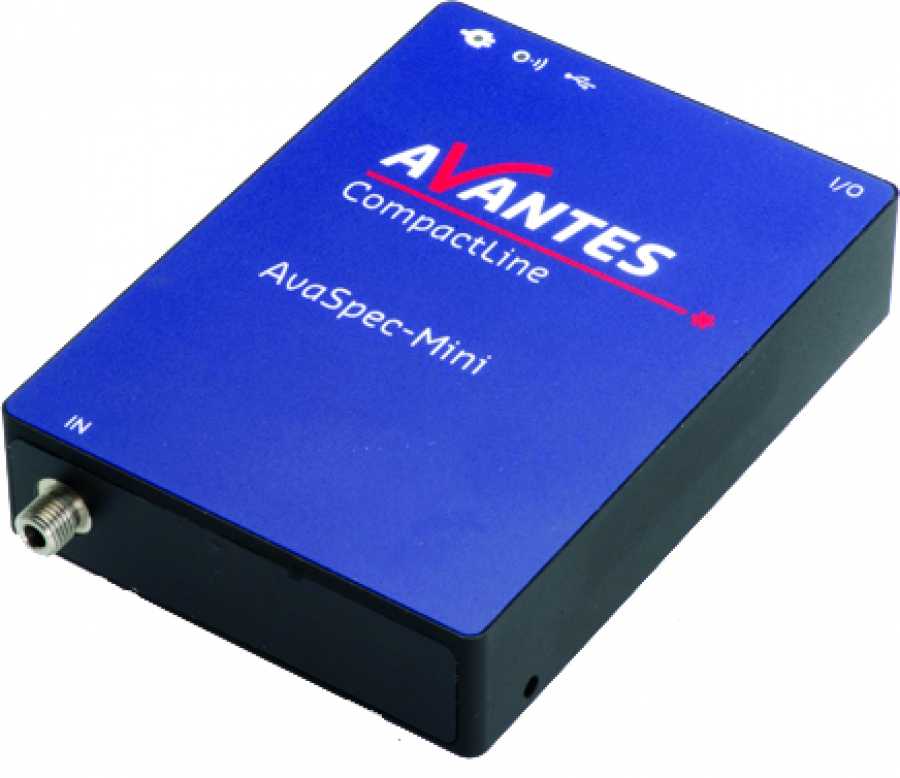
\includegraphics[width=.8\textwidth]{figures/avaspec-mini.png}
    }
  \end{minipage}
  \begin{minipage}{.49\textwidth}
    \subfloat[]{
      \centering setup sketch here
    }
  \end{minipage}
\caption[]{Spectrometer Module}
\end{figure}

\newpage
\subsection{Liquid Flux: Continuous Culture \& Turbidostat} 
\label{cult}

\paragraph{Project:} build a module consisting of media and waste bottles, 
a reactor vessel, peristaltic pump(s), and a scale; pump and scale are
controlled \textit{via} serial interfaces from an
Arduino+Touchscreen. The flow rate is controlled \textit{via} the pump
motor speed and recorded \textit{via} the scale; the flow rate is
recorded or can be set after a setup-specific (tubing) calibration
routine


\begin{enumerate}
\item \build{} a simple reactor vessel (Schott bottles) with liquid
  media flow, from media bottles through reactor vessel and out to
  waste bottle 
\item \code{}: calibration routine for the weight sensor module
\item \code{}: analog control of peristaltic motor speed and recording of
  weight loss and/or gain to record mass flow (g/min)
\item \code{}: routine to calibrate pump speed to weight loss/gain
  for a specific setup; store calibration on SD card, which allows
  to also set pump speed in g/min, or if provided with a culture
  volume, as culture dilution rate (\ph{})
\item \build{} \& \code{}: combine with \ref{spec} to make
  turbidostatic control
\item \build{}: add gassing system of project \ref{gas} to make a first
  simple bioreactor
\end{enumerate}

\paragraph{Ressources:}
\begin{itemize}
\item Arduino tutorials for
  \href{http://www.instructables.com/id/Control-peristaltic-pump-with-TA7291P-and-an-Ardui/}{Adafruit
    peristaltic pump} and general
  \href{http://playground.arduino.cc/TA7291PDCMOTORCONTROLLER/TA7291PDCMOTORCONTROLLER}{DC motor control} and \href{https://www.adafruit.com/products/1438}{Adafruit motor shield}
\item \href{http://www.elecrow.com/wiki/index.php?title=Weight_Sensor_Scales_Kit-_20KG}{Arduino library for Elecrow weight sensor kit 3 kg}
\item \href{https://cdn.sparkfun.com/datasheets/Sensors/ForceFlex/hx711_english.pdf}{HX711 24-Bit Analog-to-Digital Converter (ADC) for Weigh Scales}
\end{itemize}

\paragraph{Materials:}
\begin{itemize}
\item Bottles, screw caps with inlet/outlet openings,
  and tubing: \avail{} \& \obtain{}!
\item Scale - \obtain{}\\
  fancy:
  \href{http://de.mt.com/de/de/home/products/Industrial_Weighing_Solutions/bench-scales/weighing-platforms/high-resolution/PBK785.html}{Mettler Toledo, PBK785-3XS/f}\\cheap:
  \href{http://www.elecrow.com/weight-sensor-kit-3kg-p-883.html}{Elecrow
    Weight Sensor kit 3kg for Arduino}
\item Peristaltic pumps - \obtain{}\\ fancy:
  \href{http://www.drifton.dk/de/product/lp-bt100-2j-13/}{Longer Pump
    LP-BT100-2J, DG-2(10)}\\cheap:
  \href{http://www.ismatec.com/int_e/pumps/t_ecoline/ecomsca4.htm}{Ismatec
    Ecoline VC-MS/CA4-12}\\ cheaper: \href{Welco WPM}{Welco WPM} or
  cheapest: \href{https://www.adafruit.com/product/1150}{Adafruit}
\item Sainsmart Arduino Mega + Touchscreen - \obtain{}
\end{itemize}

\newpage
\subsection{The Server}
\paragraph{Project:} a master software running on a (detachable) linux 
desktop that synchronizes and speaks via a comon interface to all
Arduino and Raspberry Pi modules; the modules themselves can interpret
get, set and act impulses (use arguments only when absolutely
necessary).\\
During an initializiation the server may inquire what an
attached module provides (\textit{via} data IDs and SI units, meaningful
time resolution) and handle it automatically. \\
Variable higher order control or processing logics can be built
using defined data and control IDs.
\begin{enumerate}
\item \build{} combine of gas (\ref{gas}), liquid (\ref{cult})
  and light (\ref{spec}) modules into a bioreactor
\item \code{}: master program to synchronize and record data from
  the three modules
\item \code{}: combine e.g. \ref{spec} \& \ref{cult} to implement
  turbidostat control
\end{enumerate}


\paragraph{Materials:}
\begin{itemize}
\item \texttt{setTime(time\_t $t$)}: sets the current master time to
  all modules
\item \texttt{get(..., time\_t $t$)}: get all values, currently
  available (with a time stamp), or from a previous time t
%\item \texttt{set(..., time\_t $t$)}: sets specific values, now or at an
%  indicated future time $t$
\item \texttt{act(..., time\_t $t$)}: act (switch on and off, set to a
  specific value), now or at future time $t$
\end{itemize}

\newpage
\subsection{Heat Flux: Water Bath Thermostat}
\label{heat}

\paragraph{Project:} build a water bath for growth vessels, control
T, read-out energy required for maintaining constant T and estimate
the amount of heat withdrawn or administered

\begin{enumerate}
\item
\end{enumerate}

\paragraph{Materials:}
\begin{itemize}
\item Jacketed reactor vessel: \build{} or \obtain{}
\item Julabo water bath,
e.g. \href{http://www.laborhandel24.de/9162625-de?utm_source=google_shopping&gclid=Cj0KEQiA496zBRDoi5OY3p2xmaUBEiQArLNnK6uWkryhjvkNdmRLgcg2W_HIO9W1aKaKCO9gmvlkt_MaAmhe8P8HAQ}{F25-ME}
\item Arduino and/or Raspberry Pi
\end{itemize}

\newpage
\subsection{The \texttt{Kaiten Eppi}: Automated Sampling Device} 
\label{sampling}
\paragraph{Projects:} build sterile and automated sampling device; using
a controllable syringe pump, sampling into the \texttt{Kaiten Eppi}
(automated: pump sample into tubes, potentially pre-filled with
chemicals, vortex, and transport them into liquid N$_2$ or other
storage containers)

\paragraph{Materials:}
\begin{itemize}
\item Sterile sampling device by HHU glas blowers: \avail{}
\item Syringe pump: \obtain{}
\item \texttt{Kaiten Eppi}: \build{}
\item Sainsmart Arduino Mega \& Touchscreen: \obtain{}
\end{itemize}


\newpage
\subsection{Single Cell Biology: Microfluidic Device} 
\label{micro}

\paragraph{Project:} Basic microfluidics and live-cell imaging device;
scratch growth chambers and liquid flow channels into microscope slide;
attach 2--3 pumps; and control \textit{via} arduino/screen

\paragraph{Materials:}
\begin{itemize}
\item Ilka's lab microscope: \avail{}
\item Microscopy slides: \avail{}
\item 2--3 peristaltic pumps for microfluidics: \obtain{}
\item Sainsmart's Arduino Mega + Touchscreen: \obtain{}
\end{itemize}


\newpage

\section{Program}

\subsection{Day 1 $<$12:00 : Building Bioreactors}

Talks, 30-60 min:
\begin{itemize}
\item Rob's DIY Reactor - The Beginnings: The Captor -
  Arduino-controlled mini PBR
\item Dougie's DIY Reactor - 20 yrs Later
\item Avantes - Spectrometry: Spectrometry applications, incl. NIR for
  metabolite measurements and OD; software interface to Avantes
  spectrometers
\item CellDeg - Optimizing Photosynthetic Growth: Introduction to
  CellDeg's 2.5 k Euro algal growth setup (overnight 30 g/L cyano
  biomass)
\end{itemize}


\subsection{Day 1 $>$13:00 : \hack{} I}

\begin{itemize}
\item Introduction to the \gasometer{}: connecting sensors with Arduino,
  making an autonomous measurement device via Sainsmart's Touch Screen
\item Introduction to Rob's reactor: complete setup for photosynthetic growth
\item Self-organizing into teams: lab hardware (tubing etc.), control hardware
(soldering etc.), software and/or by by projects (\ref{gas}--\ref{micro}) 
\end{itemize}

\subsection{Day 2 : \hack{} II}

%Perhaps in teams, either by projects (\ref{gas}--\ref{micro}) or in
%software vs. hardware (soldering/tubing) vs. biolab (cell cultures),
%or -- most likely -- in dynamic self-organisation, working parallel on
%all projects.

\begin{itemize}
\item Hardware I: soldering, tubing
\item Software I: probe/sensor/pump $\Leftrightarrow$ arduino/raspi interfaces
\item Visit HHU's fine mechanics and glas blower work-shops, place
  orders for stuff missing for above goals
\end{itemize}

\subsection{Day 3 : \hack{} III}

\begin{itemize}
\item Hardware II: Integrate projects \ref{gas},\ref{spec}\&\ref{cult}
  into a simple DIY reactor and/or with PSI FMT150 or Multicultivator
%\item 
%\end{itemize}
%\subsection{Day 3 $>$13:00 : Consolidating}
%\begin{itemize}
\item Software II: arduino/raspi $\Leftrightarrow$  master/server interface\\
  Standard data formats and interfaces
\item Brain storming: relation of data and models and beer
%\item Beer: relation of data and models and beer
\end{itemize}

\section{Outlook: 2$^{nd}$ QTB PBR \hack{}}

\subsection{\textit{Growth Dynamics}: Photobioreactors in Research}

Talks, 30-60 min:

Nir Keren, Hellingwerf, Jan Cerveny, Dougie Murray,
something microfluidics?

\subsection{\textit{Single Cell Dynamics}: Microfluidic Devices}
Integrate project \ref{micro} with the simple microscope in
Ilka's lab, or a more advanced system (CAi?)

%\subsection{Growth Dynamics}

\subsection{\textit{Omics}: Sterile and Automated Sampling Devices}

Proper sampling for high-throughput data (mass spectrometry, sequencing)
acquisition

\end{document}
